\documentclass[]{article}
\usepackage{graphicx}
\usepackage[T1]{fontenc}
%\usepackage[utf8]{inputenc}
\usepackage[spanish]{babel}
\usepackage{listings}
\pagenumbering{gobble}
%opening
\title{Exposición}
\author{Carolina Jijón Romero
y David Alonso Garduño Granados}
\usepackage{tikz,stackengine}
\usepackage{pgfplots}
\date{Diciembre 10 del 2019}
\begin{document}

\maketitle

\section{Sympy}
Sympy es una biblioteca de Python para utilizar matemática simbólica, es de acceso libre y se espera que llegue a ser un sistema de álgebra por computadora, que mantenga un código simple para ser légible y extensible por casi cualquier usuario.
Una de las ventajas es que está escrito sobre Python y usa a Python como su lenguaje, lo que hace sencillo su funcionamiento si ya conoces un poco sobre Python.

Para comenzar a usarlo busqué algunos tutoriales y me cautivó enseguida, su funcionamiento y versatilidad es impresionante, algo que me pareció asombroso es que todas las expresiones que obtengamos o que trabajamos en Sympy podemos llevarlas a LaTeX con un solo comando.
No encontré nada de Sympy en la wiki de WXPython así que todos los ejemplos que plantee son míos.

Primero definimos los símbolos, letras sin un valor numérico definido y, que por defecto, están en el campo de los número complejos, esta última propiedad puede ser modificada desde la hipótesis, con assumptions0 verificamos las propiedades de ese símbolo.
\vfill
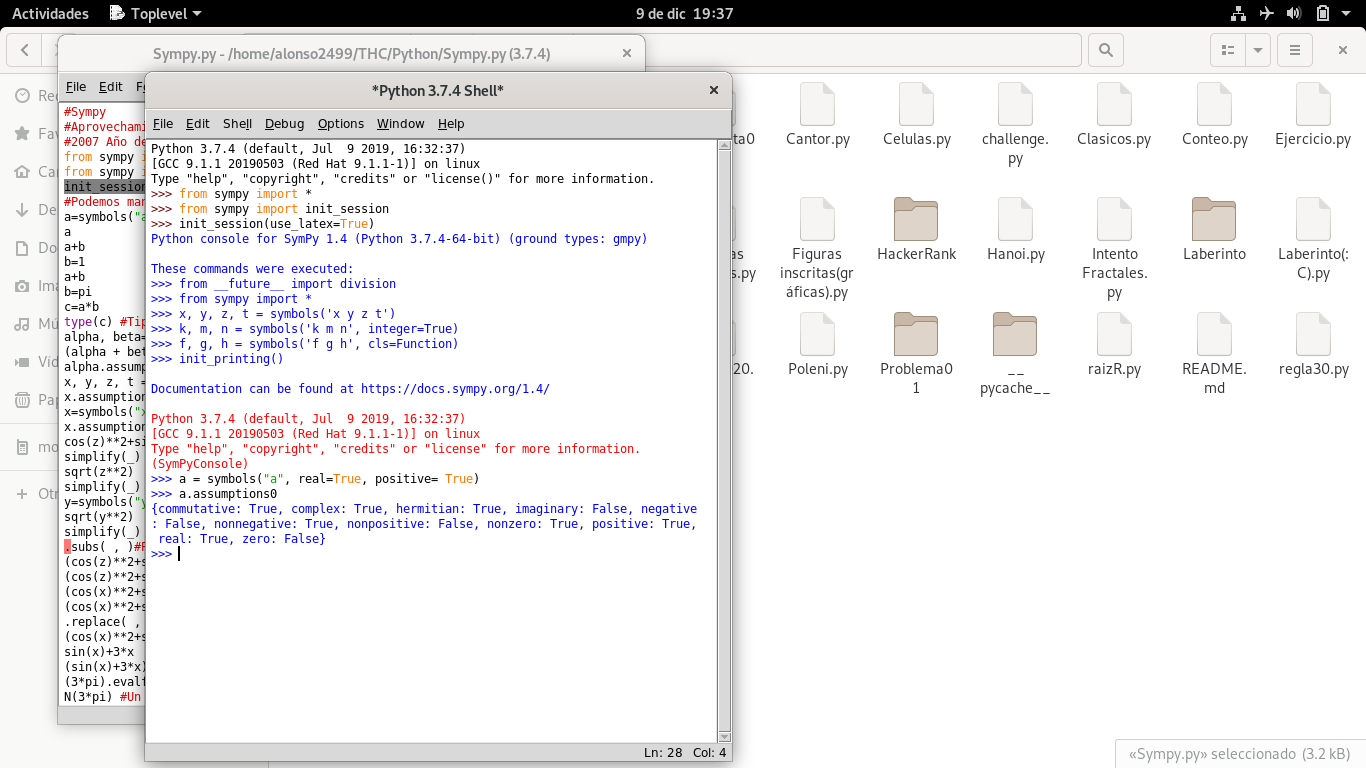
\includegraphics[scale=0.20]{Imagenes/SPY1.png}
\vfill
Con esto podemos comenzar a imaginar el potencial de Sympy con las facilidades de Python. Todo lo que se trabaja despues lo importé a LaTeX con print(latex(\_), como lo muestra la siguiente imagen:

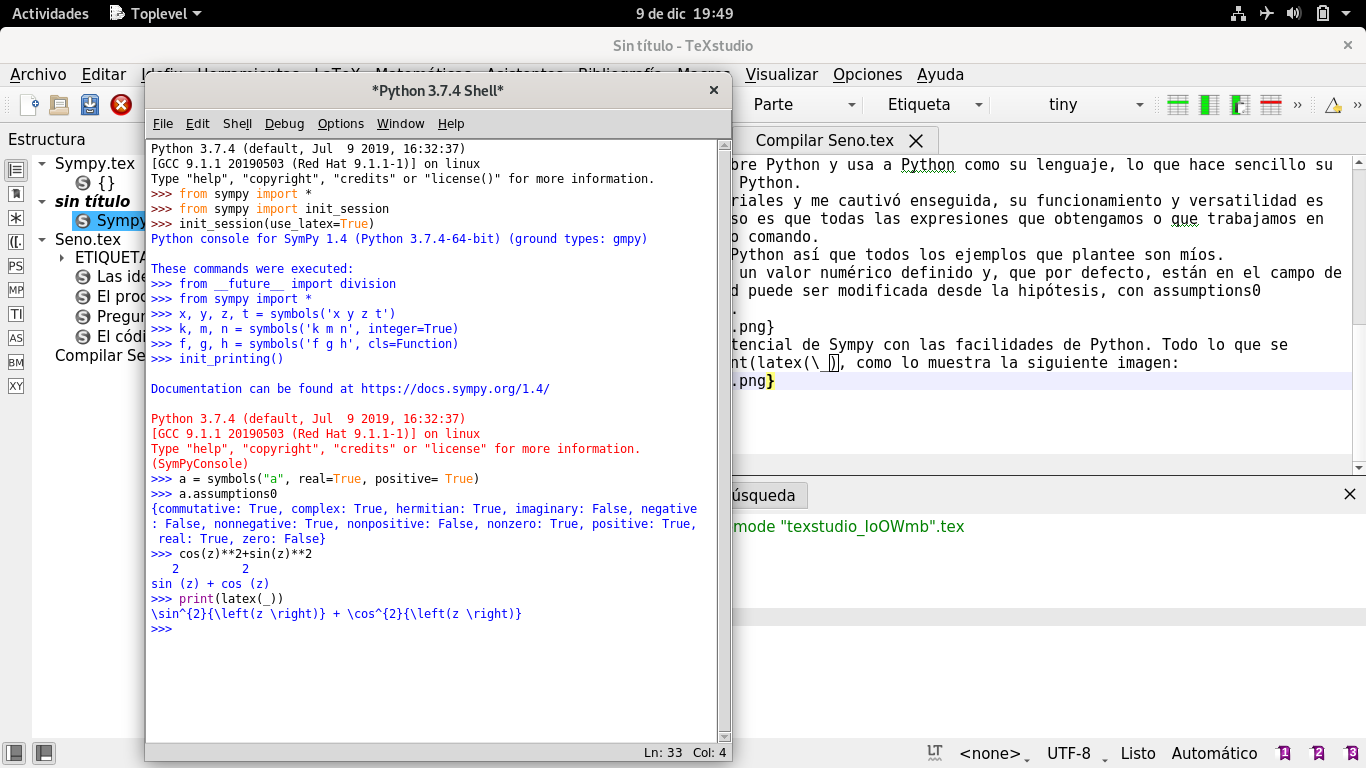
\includegraphics[scale=0.20]{Imagenes/SPY2.png}

Así se ve el comando que nos regresa:

$ \sin^{2}{\left(z \right)} + \cos^{2}{\left(z \right)} $

En el código comenté y presenté las características más importantes de Sympy, las conseguí línea por línea así que deberán de ser ejecutadas así, además fueron ejemplos de mi creación.

En conclusión en esta parte, Sympy es una potente extensión de Python, además me gustó pues se acomoda muy bien a mi carrera <3, la forma de procesar las expresiones matemáticas tiene mucho potencial.
\section{FLTK}
Para esta sección las complicaciones se dieron desde el momento de su instalación, pero después de una larga búsqueda sobre como instalarlo y un par de consultas puedo mencionar los pasos que usé para instalar esta biblioteca:

	-Primero instalar FLTK con sus bibliotecas de desarrollo, o los comandos "sudo dnf install fltk", "sudo yum install fltk-devel".
	
	-Con todo esto listo, descargar de la página de internet pyFLTK el archivo comprimido que contiene los archivos para instalarlo en Python, ya con el archivo, descomprimirlo y después correr el setup.py de la siguiente forma: "sudo python3 setup.py build install".
	
	El proceso para encontrar esta solución llevó otros pasos que tal vez omití, ya que encontrarla del todo me costó mucho tiempo y paciencia.
	
FLTK es un entorno gráfico que puede ser trabajado en muchos lenguajes de programación, no es nativo de Python. Genera entornos gráficos interactivos.

Aprendí la parte básica de pyFLTK, el como hacer ventanas con dimensiones y títulos predeterminados, hasta como hacer ventanas con texto en buffer que se edita en una y se muestra en otra, el potencial gráfico e interactivo de esta herramienta solo se podrá descubrir ensayando con ella ya que su manipulación en python es muy específica y todo debe ser explícito.

Conseguí un par de ejemplos comentados en el codígo con el nombre FLTK, y construí el ejemplo basado en lo que encontré.
\end{document}
